\documentclass[a4paper,12pt]{article} %style de document                        
\usepackage[utf8]{inputenc} %encodage des caractères                            
\usepackage[french]{babel} %paquet de langue français                           
\usepackage[T1]{fontenc} %encodage de la police                                 
\usepackage[top=2cm,bottom=2cm,left=2cm,right=2cm]{geometry} %marges            
\usepackage{graphicx} %'affichage des images                                    
\usepackage{verbatim}
\usepackage{enumitem}
\usepackage{amssymb}
\usepackage{perpage}
\MakePerPage{footnote}
\usepackage[colorlinks=true,linkcolor=blue,urlcolor=teal]{hyperref}
\begin{document}
\renewcommand{\contentsname}{Sommaire}
\title{Projet de Conception Logiciel }
\author{Mathieu \textsc{Goudal},Clément \textsc{Bartolone},Guillaume \textsc{Lericheux}, Brice \textsc{Andrieux}}
\date{2023}
\maketitle
\begin{center}

\includegraphics[scale=0.5]{images/UNICAEN.png}
\end{center}

\newpage
\tableofcontents
\newpage
\section{Introduction}
L'objectif de ce projet et de concevoir un jeu avec des pièces dans le même style que Tetris.
Le but du jeu est de modifier la positions des pièces d'un état initial aléatoire et en faire un bloc compact qui prendra le moins de place possible dans le plateau de jeu .
Ce projet est bien évidemment MVC et utilise plusieurs design patterns (voir \ref{Design Factory}, \ref{design chain} et \ref{design IA})

\section{Modèle}
Le Modèle est la base du projet : il permet à la vue de changer d’état à l'aide d'écouteurs et via le soutien du contrôleur.
\subsection{Pièce}
Les pièces sont les éléments avec lesquels le joueur va pouvoir interagir afin de pouvoir déterminer son score .
\subsubsection{Matrice}
Chaque pièce est caractérisée par sa taille, sa position sur un plateau et une Matrice de booléens.\\
Chaque case à l'état : "True" dans la matrice signifie qu'une partie de la pièce est présente à l'endroit indiqué .\\
Et inversement à l'état : "False" cela signifie que la pièce n'est pas pas présente à cette position.
Exemple : 
\begin{center}
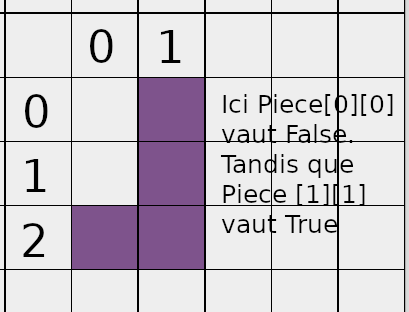
\includegraphics[scale=0.5]{images/Piece1.png}
\end{center}
\subsubsection{Rotation}
Il est possible pour chaque pièce de faire une rotation de 90 ou -90° degrés.
Sur notre projet nous avons opté pour une solution plus efficace qu'une rotation de matrice.\\
Pour ce faire il faut modifier le getter de position, de cette manière si l'on utilise la fonction getRotatedCoord(X,Y) avec une rotation de 180 alors la fonction n'ira pas chercher si la valeur est True en Piece[x][y] mais plutôt en Piece[(tailleX-1)-x][(tailleY-1)-y].\\
La rotation se fait donc en temps constant .
\subsection{Création de Pièce et Design Pattern Factory}
\label{Design Factory}
La création de pièce s'effectue dans notre projet grâce au pattern Factory. L'idée est de rendre la création d'une pièce plus pratique, ce pourquoi nous avons créé un \textbf{PieceBuilder} qui permet de choisir chaque attribut d'une pièce avant sa création, qui sont :
\begin{itemize}
    \item Ses coordonnées.
    \item Sa taille.
    \item Sa rotation.
    \item Sa forme.
    \item Sa couleur.
\end{itemize}

Il est aussi possible de générer une pièce aléatoire en fournissant les arguments nécessaires comme la taille maximale, minimale,la position maximale, etc... \\
Quand tout a été spécifié il suffit d'appeler \textbf{Build()} pour générer la pièce.

\subsection{Plateau de jeu}
Le plateau de jeu est l'une des classes du projet les plus importantes , il doit gérer :
\begin{itemize}
    \item L'initialisation des pièces .
    \item L'ajout des pièces .
    \item Le déplacement des pièces.
    \item Le calcul du score.
\end{itemize}
\subsubsection{Matrice}
Dans le plateau on retrouve un tableau de boolean, cela permet de faciliter l'usage de nombreuses fonctions ainsi que la vue.\\
Le principe reste le même que celui des pièces , il est juste plus global et prend en compte toutes les pièces. 
\subsubsection{Résultat}
La fonction pour calculer le résultat est assez simple :\\
Il faut parcourir les pièces pour pouvoir prendre respectivement les positions X,Y les plus petites et les plus grandes où une pièce se trouve afin de constituer un rectangle dont on calculera l'aire (Longueur * Largeur), ce qui est le score pour cet état du plateau.
\subsection{Ajout de pièce et Design Chain of Responsibility}
\label{design chain}
La fonction ajouterPiece(Piece) va créer une Chain of Responsibility. 
Pour ajouter une pièce il faut vérifier plusieurs étapes et dans le cas où une étape n'est pas correcte la pièce ne peut pas être placée.\\
Dans ce cas présent on à deux types de maillons qui s'assembleront pour faire une chaîne.
\subsubsection{Maillon de tête / Maillon Hors Jeu}
Il s'agit du premier maillon de la chaîne comme tout les autres maillons si celui la est faux la chaîne s’arrête et les autres maillons ne sont pas visités .\\
Ce maillon est assez simple à comprendre, si la pièce sort du plateau alors la pièce ne peut pas être ajoutée .\\
\subsubsection{Maillon Collision}
Ce maillon correspond au reste de la chaîne. Chacun de ces maillons correspond à une pièce déjà placé sur le plateau, et regarde si une collision a lieu avec la pièce que l'on souhaite placer. \\
Il vérifie alors plusieurs cas afin de réduire la complexité de l'algorithme :\\
Premièrement : il faut vérifier que les deux rectangles qui entourent chacune des deux pièces soit en collision. Dans le cas contraire il est impossible qu'il y ait une collision des deux pièces, donc ce maillon sera correct.\\
Deuxièmement : il faut prendre le plus petit rectangle commun entre deux pièces,  et itérer dessus afin de vérifier qu'aucune de ces cases contiennent une partie de chaque pièce pour que le maillon soit correct.\\
Si tout les maillons sont correct alors la pièce peut être ajoutée . Si un seul ne l'est pas, on arrête la chaîne et la pièce ne pourra pas être placé ici.\\
\subsection{Initialisation du Plateau et Design Strategy}
L'initialisation du plateau est générée avec plusieurs classes déjà existantes : 
\begin{itemize}
\item Le PieceBuilder afin de générer des pièces aléatoires .
\item Le PlateauPuzzle et sa fonction ajouterPiece().
\end{itemize}
Le design pattern Strategy a pour objectif de séparer plusieurs options de ce que l'on souhaite faire en classes à part entière, toutes sous une même classe ou interface qu'elles héritent ou implémentent.
Dans notre situation les classes du design pattern sont caractérisées par le type de pièces qui doivent être générées.
\begin{itemize}
\item GenRandAll génère un plateau rempli de pièces aléatoires.
\item GenRandU génère un plateau rempli de pièces en forme de U.
\item GenRandS génère un plateau rempli de pièces en forme de S.
\item etc etc ...
\end{itemize}
Le fonctionnement des GenRand est simple: \\
On donne en argument de la fonction GenRand :  
\begin{itemize}
\item Un plateau déjà initialisé.
\item Un nombre de pièces qui sera généré sur le plateau.
\item Une difficulté qui augmente la taille maximum des pièces.
\end{itemize}

Enfin il existe une variable "autoloop" qui bloque la génération si ajouterPiece a échoué 100 fois de suite pour éviter de  faire tourner l'algorithme  en boucle.
La difficulté fait varier la taille maximum des pièces (plus les pièces sont petites plus il est facile de faire un score bas...).

\section{Menu}
Le \textbf{Menu} permet d'initialiser une partie en créant un \textbf{PlateauPuzzle} contenant 10 pièces. Au lancement du Menu une fenêtre s'ouvre et vous avez 3 choix de difficultés :

\begin{itemize}
    \item \textbf{Facile}
    \item \textbf{Moyen}
    \item \textbf{Difficile}
\end{itemize}

\begin{figure}[ht]
    \centering
    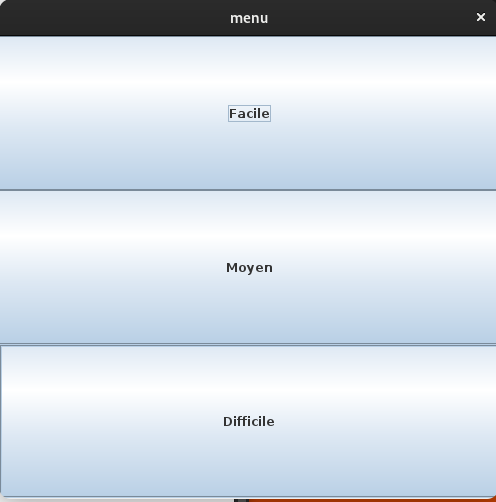
\includegraphics[width=0.5\linewidth]{images/manu.png}
    \caption{menu}
\end{figure}


\section{Contrôleur}
\subsection{ControllerJoueur}
Après avoir sélectionné la difficulté via le menu, il vous sera demandé si vous voulez faire jouer une IA.

\begin{figure}[ht]
    \centering
    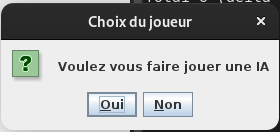
\includegraphics[width=0.5\linewidth]{images/choixJoueur.png}
    \caption{menu}
\end{figure}

Si vous sélectionné oui alors le jeu est lancé et l'IA effectue ses coups (vous ne pouvez rien contrôler) et si vous sélectionné non alors c'est à vous de jouer.

\subsection{Intelligence Artificielle}
\label{design IA}
L'implémentation de l'intelligence artificielle dans ce projet se base sur le Pattern Strategy : on a une classe "client" (ici, ClientIA) qui va appeler une instance d'une interface ou classe abstraite "strategy" (ici, c'est la classe abstraite StrategyIA), qui peut avoir plusieurs implémentations (ici, BasiqueIA et MoinsBasiqueIA).

\subsubsection{BasiqueIA}
Basique IA va essayer de déplacer chacune des pièces qui sont les moins bien placés (autrement dis, celles qui sont les plus au bords de chaque coté du plateau), et essayer de mieux les placer, c'est à dire les éloigner du bord dont elles étaient proche. \\
On peut alors décomposer son fonctionnement en plusieurs étapes :
\begin{itemize}
    \item Pour chaque bord possible (haut,droit,bas et gauche), on prend toutes les pièces qui en sont les plus proche.
    \item Pour chaque pièce sélectionné si dessus, on essaie de l'éloigner du bord qui lui correspondais.
    \item On continue ces actions tant qu'une des conditions de fin n'est pas atteinte. 
\end{itemize}
 Les conditions de fin de cet IA sont :
\begin{itemize}
    \item Le nombre de déplacements limite défini à l'avance a été atteint. Il est possible qu'il n'y ait pas de limite, auquel cas cette condition n'aura jamais lieu.
    \item On a essayé de déplacer chacune des pièces les plus proches de chaque bord sans succès.
    \item On a essayé de déplacer chacune des pièces les plus proches de chaque bord, 3 fois, sans améliorer le score.
\end{itemize}

Cette IA est donc capable de rapprocher les pièces les une des autres pour améliorer le score, mais elle ne peut pas détecter un meilleur emplacement pour une pièce si cela nécessite un déplacement dans chaque axe, et ne peut pas non plus faire tourner les pièces.

\subsubsection{MoinsBasiqueIA}
Moins Basique IA, comme indique son nom, est moins basique que Basique IA.
Elle garde le même principe que Basique IA en essayant juste d'éloigner les pièces les plus proche de chaque bord, mais contrairement à celle ci, elle est capable de mouvements sur les 2 axes et de faire tourner les pièces. \\
On peut aussi décomposer son fonctionnement en plusieurs étapes :
\begin{itemize}
    \item Pour chaque bord possible (haut,droit,bas et gauche), on prend toutes les pièces qui en sont les plus proche.
    \item Pour chaque pièce sélectionné si dessus, on essaie de l'éloigner du bord qui lui correspondais :
    \item Pour chaque rotation possible, pour chaque mouvement latéral au bord que l'on peut faire sans atteindre les bords latéraux, on essaie d'éloigner la pièce du bord. Si un déplacement a lieu, on n'essaie pas de faire les suivant.
    \item On continue ces actions tant qu'une des conditions de fin n'est pas atteinte. 
\end{itemize}

Les conditions de fin de cet IA sont les mêmes que pour Basique IA. \\

Cette IA est donc bien plus apte à trouver une solution proche du plus optimal possible que Basique IA, mais en contrepartie elle prend plus de temps pour fonctionner. \\
\textbf{A noter que} dans notre implémentation actuelle, Moins Basique IA provoque parfois une \textit{Exception in thread "AWT-EventQueue-0" java?util.ConcurrentModificationException} . Cela ne semble pas nuire au fonctionnement de l'IA, néanmoins pour cette raison nous avons préféré ne pas permettre à l'utilisateur d'utiliser cette IA sans modifier le main, et donc seul l'IA Basique est disponible sans action sur le code.

\subsection{Contrôleur Terminal}
Le Contrôleur Terminal permet de jouer au jeu depuis un terminal.
Son fonctionnement est divisé en plusieurs actions qui on chacune leurs utilités,
et chaque action est accessible grâce a une lettre . \\
De plus le contrôleur est contenu dans son propre thread afin de permettre
son utilisation asynchrone du reste du programme comme l'interface swing.

\begin{figure}[ht]
    \centering
    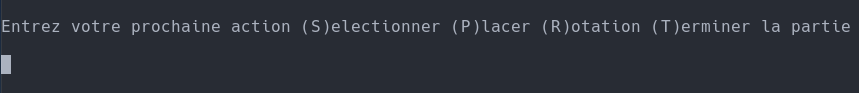
\includegraphics[width=0.5\linewidth]{images/controleurterminal1.png}
    \caption{menu du terminal en pleine partie}
\end{figure}

\subsubsection{Action "Sélectionner"}
L'action \textbf{Sélectionner} permet de sélectionner une pièce, pour ce faire, le contrôleur nous demande dans un premier temps de sélectionner l'action elle même : il suffit de presser "S" ou "s" pour utiliser cette action. \\
Dans un deuxième temps le contrôleur nous demande de sélectionner une coordonnée où placer le bloc il faut alors rentrer une coordonnée Horizontale puis Verticale, s'il existe une pièce a cette coordonnée, elle est sélectionnée
sinon on redemande a l'utilisateur de rentrer une coordonnée.
\subsubsection{Action "Placer"}
L'action \textbf{Placer} permet de placer la pièce sélectionnée sur le plateau, évidemment cela ne fonctionne que si il existe une pièce sélectionnée
encore une fois il faut choisir l'action dans le menu cette fois si avec la l'entrée "P" ou "p", comme la dernière action on demande a l'utilisateur de
choisir une coordonnée Horizontale puis Verticale et ensuite on essaie de placer, si c'est possible on la place et on passe a la prochaine action, sinon
on notifie l'utilisateur de son erreur et on lui redemande de choisir une coordonnée.
\subsubsection{Action "Rotation"}
l'action de \textbf{Rotation} permet de faire tourner la pièce sélectionnée, encore une fois cela ne peux pas fonctionner si il n'y a pas de pièce
sélectionnée, la sélection de l'action se fait avec "R" ou "r" par défaut la rotation s'effectue a droite, il est possible de changer le sens de rotation
en écrivant "RD" ou "RG" (ainsi que toutes les variation sans majuscules) cela effectuera une rotation dans le sens désiré et la prochaine rotation "R" ou "r"
s'effectuera dans le même sens.
\subsubsection{Action "Terminer"}
l'action de \textbf{Terminer} permet de finir la partie, cela n'est pas possible si une pièce est sélectionnée, ça serait de la triche! On y accède en choisissant l'option "T" ou "t".
\section{Vue}
\subsection{VueTerminal}
La vue terminal permet de visualiser la partie dans le terminal, quand la partie est lancée, la vue se met à jour, ce qui permet de voir la partie. \\
L'interface avec le contrôleur ressemble a ceci:
\begin{figure}[ht]
    \centering
    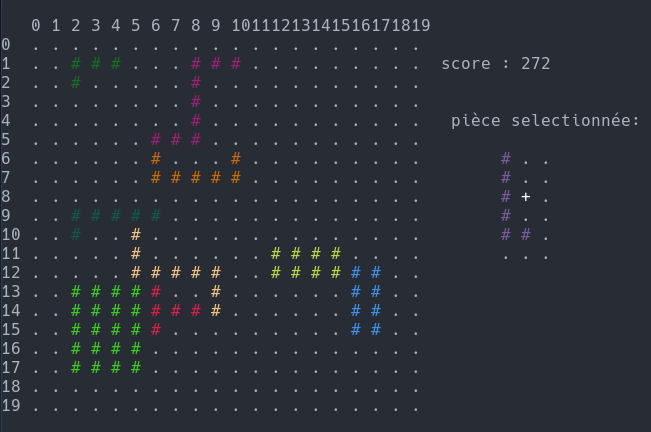
\includegraphics[width=0.5\linewidth]{images/vueterminal1.png}
    \caption{Vue terminal en pleine partie}
\end{figure}

A gauche il y a le plateau de jeu avec les lignes et colonnes numérotées afin de simplifier la partie pour le joueur.
A droite est affiché le score pour le plateau de jeu actuel, la pièce sélectionnée n'étant pas compté étant donné qu'elle est comme hors du jeu, mais il faut la placer avant de finir la partie donc on ne peux pas tricher!\\
En dessous du score est affiché la pièce sélectionnée, elle est dans sa propre grille où un "+" représente le centre quand il n'y a pas de bloc dessus, sinon c'est une croix "X".

\section{Interface graphique}

\subsection{Vue}

\subsubsection{DrawPiece}
La classe \textbf{DrawPiece} prend en argument un \textbf{PlateauPuzzle}. Elle permet d'afficher dans la fenêtre la pièce sélectionnée par le joueur et elle contient le bouton \textbf{resultat} qui va permettre au joueur de mettre fin à la partie et de récupérer son score. 

\begin{figure}[ht]
    \centering
    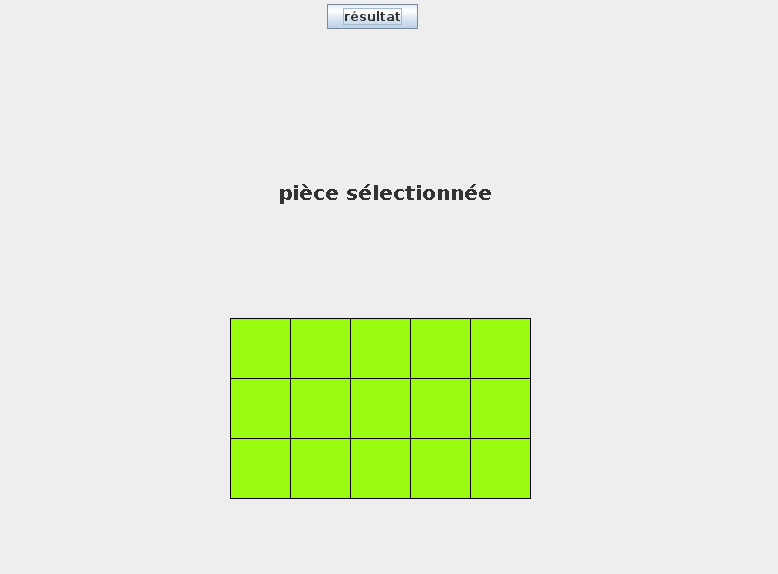
\includegraphics[width=0.5\linewidth]{images/pieceSelect.png}
    \caption{Vue de DrawPiece pendant une partie}
\end{figure}

Quand le joueur clic sur le bouton résultat une pop-up apparaît à l'écran lui indiquant son score et que la partie est terminé.  

\begin{figure}[ht]
    \centering
    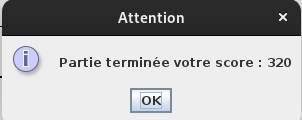
\includegraphics[width=0.5\linewidth]{images/endGame.png}
    \caption{pop-up de fin de partie}
\end{figure}

Si le joueur clic sur le bouton alors qu'une pièce est sélectionnée alors un message différent apparaît.

\begin{figure}[ht]
    \centering
    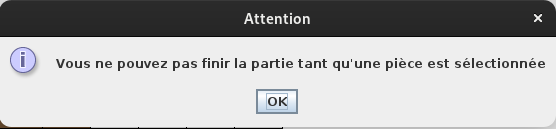
\includegraphics[width=0.5\linewidth]{images/erreurEndGame.png}
    \caption{pop-up d'erreur de fin de partie}
\end{figure}

\subsubsection{DrawPlateau}
La classe \textbf{DrawPlateau} prend en argument un \textbf{PlateauPuzzle}. Elle permet de dessiner le plateau de jeu.

\begin{figure}[ht]
    \centering
    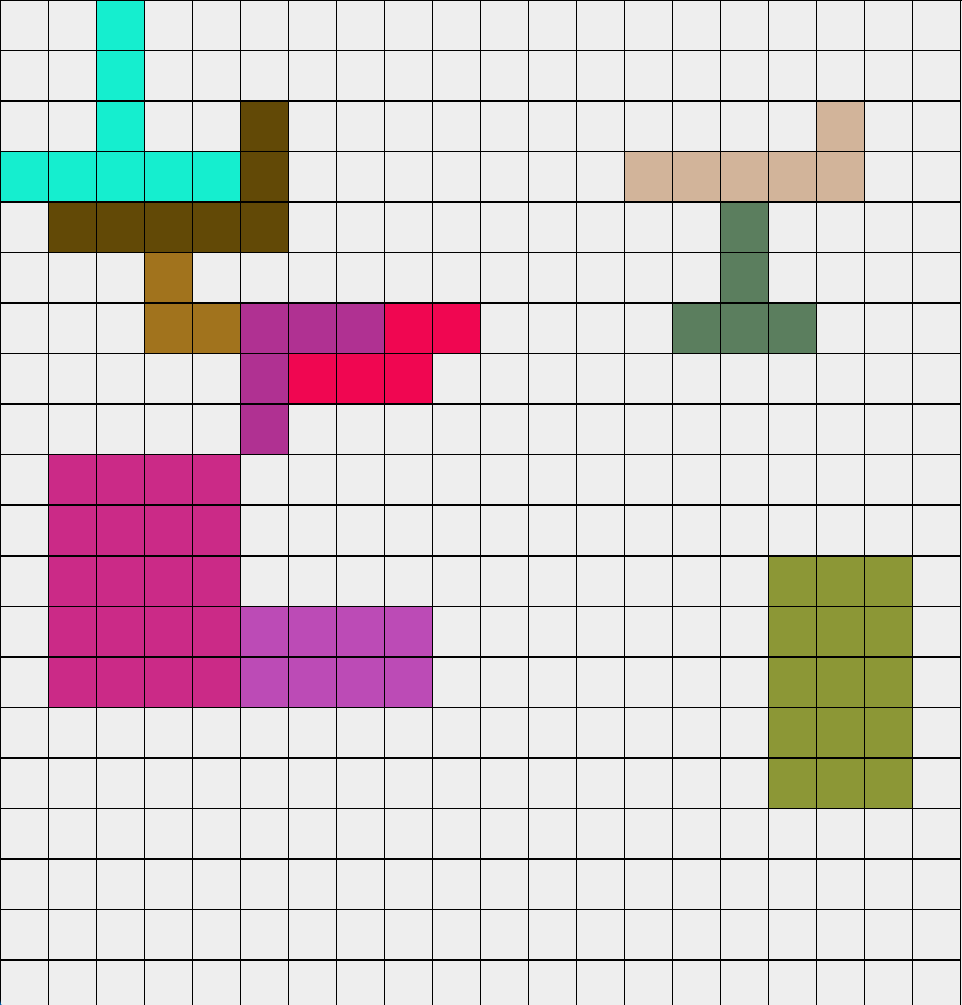
\includegraphics[width=0.5\linewidth]{images/plateauInterface.png}
    \caption{Vue de DrawPlateau pendant une partie}
\end{figure}

\subsection{Interface}
La classe \textbf{Interface} prend en argument un \textbf{PlateauPuzzle}. Elle permet d'initialiser \textbf{DrawPlateau} ainsi que \textbf{DrawPiece}, elle crée une \textbf{JFrame} et lui ajoute le contenu de \textbf{DrawPlateau} et de \textbf{DrawPiece}.

\begin{figure}[ht]
    \centering
    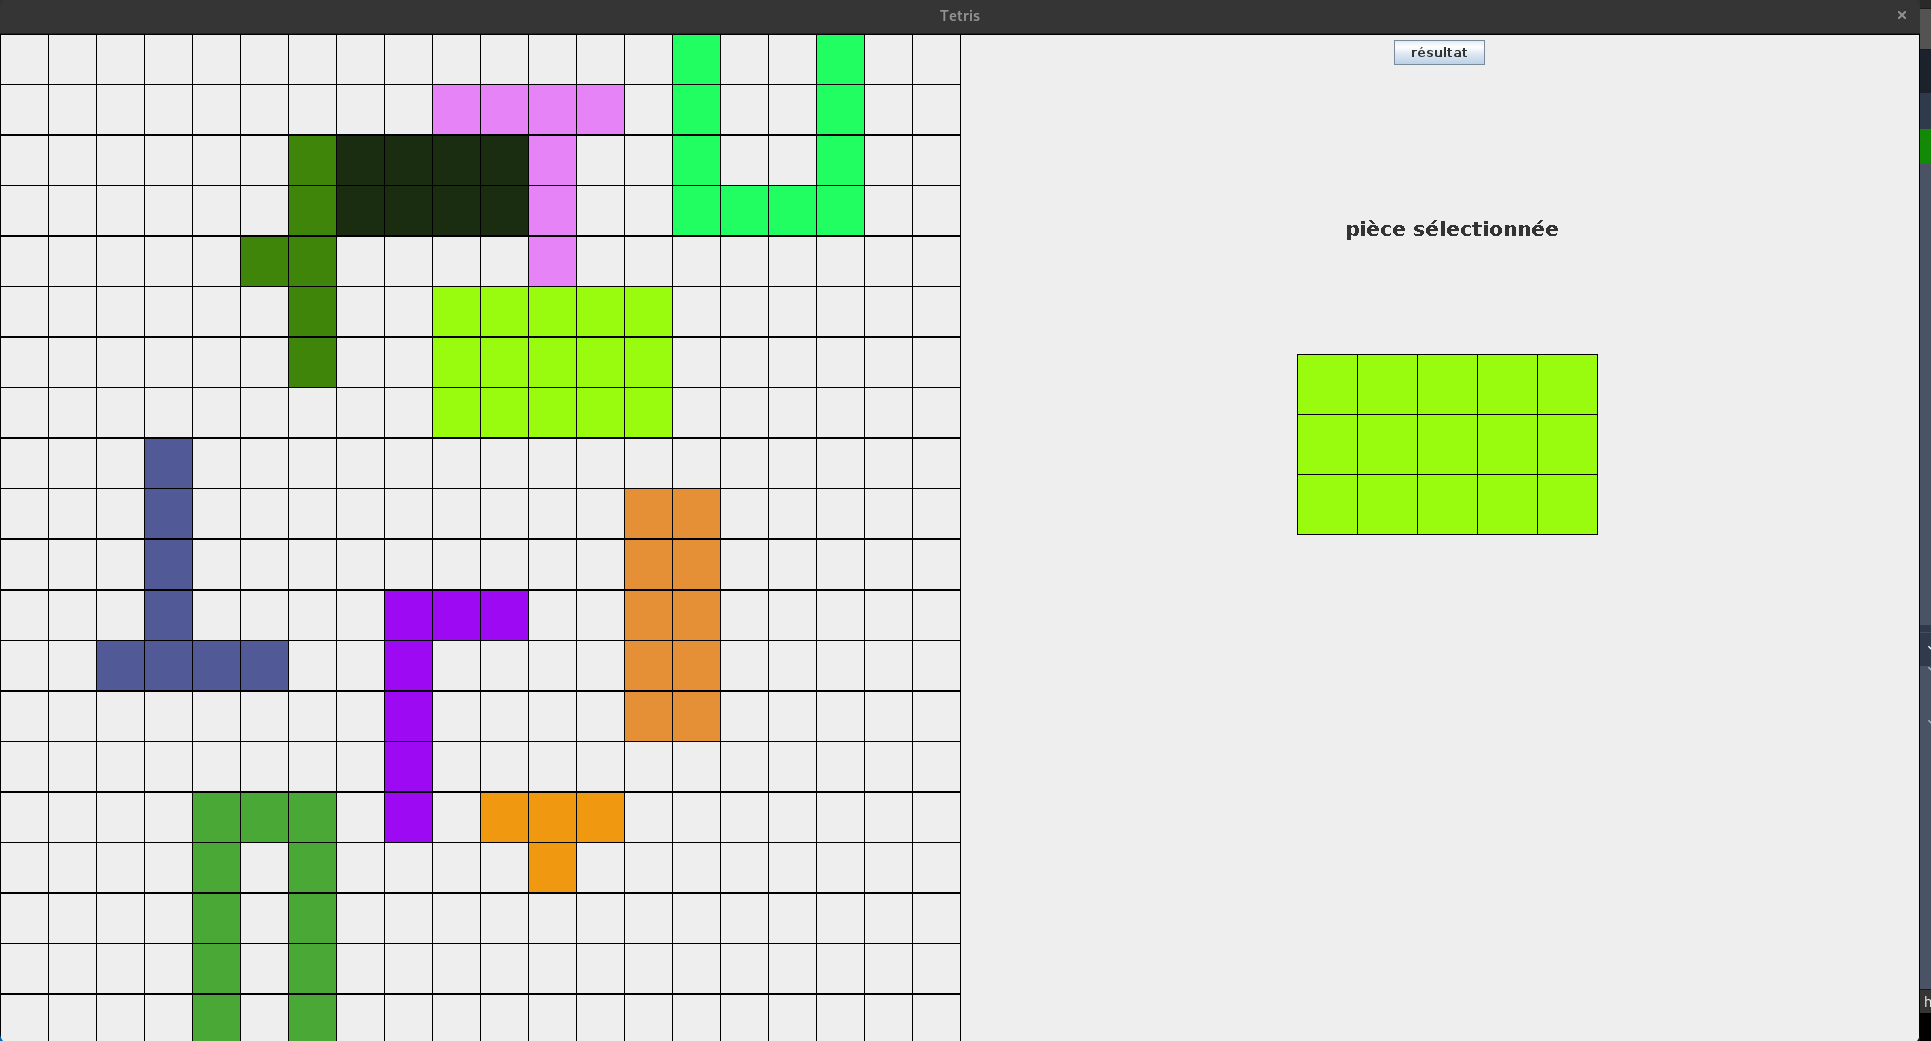
\includegraphics[width=0.5\linewidth]{images/partie.png}
    \caption{Vue de de l'interface pendant une partie}
\end{figure}

\par Chaque classe de la vue implémente la classe \textbf{Ecouteur}. Ainsi, dès qu'il y a un changement dans le plateau, la vue est averti et elle se met à jour.

\subsection{ControllerInterface}
Le \textbf{ControllerInterface} prend en argument \textbf{DrawPlateau} et \textbf{DrawPiece}. \textbf{Attention}, le controller ne sert absolument pas à afficher quoi que ce soit il à besoin de ces deux classes en argument dans le seul et unique but de leur ajouter des \textbf{MouseListener} et des \textbf{MouseMotionListener}.

\subsubsection{ControllerPiece}
Le \textbf{ControllerPiece} prend en argument \textbf{DrawPiece}. Il sert uniquement à ajouter un \textbf{ActionListener} sur le bouton résultat contenu dans \textbf{DrawPiece}.

\subsubsection{ControllerPlateau}
Le \textbf{ControllerPlateau} prend en argument \textbf{DrawPlateau}. Il sert à implémenter les différents événements liés à la souris. Il y a 3 événements :

\begin{itemize}
    \item \textbf{Le clic gauche}
    \item  \textbf{Maintenir le clic gauche/droit}
    \item  \textbf{Le clic droit}
\end{itemize}

\subsubsection{Le clic gauche}
Le clic gauche permet simplement de sélectionner une pièce. Pour sélectionner une pièce, il suffit de cliquer dessus. Si vous avez un doute sur le fait que la pièce cliqué est bien sélectionnée, il vous suffit de regarder à droite de l'écran dans l'espace "pièce sélectionnée".

\subsubsection{Maintenir le clic gauche/droit}
Le fait de maintenir le clic gauche/droit ne fonctionne que si au préalable vous avez sélectionné une pièce. Une fois que vous avez sélectionné une pièce, vous pouvez la déplacer en maintenant le clic gauche/droit. Une fois que vous relâchez le clic, la position de la pièce sera modifiée dans le plateau et elle sera automatiquement désélectionnée.

\subsubsection{Le clic droit}
Le clic droit permet de faire effectuer une rotation à n'importe quelle pièce du plateau (pas forcément la pièce sélectionnée). Si la rotation ne peut pas s'effectuer car il y aura une collision avec une autre pièce, une fenêtre pop-up apparaîtra vous indiquant que la rotation n'est pas possible à cet endroit.

\begin{figure}[ht]
    \centering
    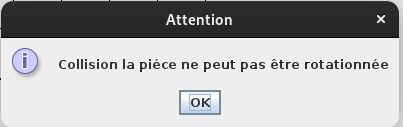
\includegraphics[width=0.5\linewidth]{images/erreurCollision.png}
    \caption{pop-up d'erreur lors d'une rotation}
\end{figure}


\end{document}

